\documentclass[12pt,a4paper]{article}
\usepackage[utf8]{inputenc}
\usepackage{amsmath, amssymb}
\usepackage{graphicx}
\usepackage{geometry}
\usepackage{float}
\usepackage{booktabs}
\usepackage{circuitikz}
\usepackage{caption}
\usepackage{subcaption}
\usepackage{enumitem}
\setlist{itemsep=2pt, parsep=1pt, topsep=3pt}
\geometry{a4paper, margin=1in}

\title{\textbf{OP-AMP Frequency Response and Mathematical Tools}}
\author{Yamulapalli Nandu Navadeep \\ Roll Number: IMS24267}
\date{Date of Experiment: 07/10/2026 \\ Date of Submission: 15/10/2026}

\begin{document}

\maketitle

\section{Name of the Experiment}
OP-AMP Frequency Response and Mathematical Tools (Inverting, Non-Inverting, Adder, Subtractor, Differentiator, and Integrator).

\section{Aim of the Experiment}
\begin{enumerate}
    \item To study the frequency response of an operational amplifier (IC 741) in both inverting and non-inverting configurations and determine their respective bandwidths and Gain-Bandwidth Products (GBWP).
    \item To construct and analyze basic analog mathematical computing circuits using IC 741, including an adder, a subtractor, an active differentiator, and an active integrator, and observe the resulting waveforms on the oscilloscope.
\end{enumerate}

\section{Theory}
An operational amplifier (op-amp) is a direct-coupled, high-gain differential voltage amplifier featuring two input terminals and a single-ended output. The terminal marked `$-$' is the inverting input, while the terminal marked `$+$' is the non-inverting input. An ideal operational amplifier possesses infinite open-loop gain ($A_{OL} \to \infty$), infinite input impedance ($R_{in} \to \infty$), zero output impedance ($R_{out} = 0$), infinite bandwidth, and zero input offset voltage.

In practical analog circuits, negative feedback is applied to stabilize the gain, increase circuit bandwidth, and achieve predictable linear performance determined almost entirely by external passive components.

\subsection{Inverting Amplifier}
In the inverting configuration, the non-inverting terminal is connected to ground, and the input signal $V_i$ is fed to the inverting terminal through an input resistor $R_1$. A feedback resistor $R_F$ connects the output back to the inverting input. Because the open-loop gain is extremely large and no current enters the op-amp input terminals, the potential at the inverting terminal is held at virtual ground ($V_- \approx V_+ = 0$).

Applying Kirchhoff's Current Law (KCL) at the inverting summing node gives:
\begin{equation}
    \frac{V_i - 0}{R_1} + \frac{V_o - 0}{R_F} = 0
\end{equation}
Solving for the closed-loop voltage gain yields:
\begin{equation}
    A_{v,\text{inv}} = \frac{V_o}{V_i} = -\frac{R_F}{R_1}
\end{equation}
The negative sign signifies a $180^\circ$ phase inversion between the output and input signals.

\subsection{Non-Inverting Amplifier}
In the non-inverting configuration, the input voltage $V_i$ is applied directly to the non-inverting terminal ($+$). The feedback network ($R_F$ and $R_1$) forms a potential divider from the output to ground, feeding a fraction of the output back to the inverting terminal ($-$).

By virtual short-circuit condition, $V_- \approx V_+ = V_i$. Applying KCL at the inverting node:
\begin{equation}
    \frac{0 - V_i}{R_1} + \frac{V_o - V_i}{R_F} = 0
\end{equation}
Solving for the voltage gain gives:
\begin{equation}
    A_{v,\text{non}} = \frac{V_o}{V_i} = 1 + \frac{R_F}{R_1}
\end{equation}
The output is in phase with the input, and the gain is always greater than or equal to unity.

\subsection{Frequency Response and Gain-Bandwidth Product}
Internally compensated general-purpose operational amplifiers, such as the IC 741, incorporate an internal compensation capacitor (typically $30\text{ pF}$) to prevent spontaneous high-frequency oscillations. This internal capacitor introduces a dominant pole at a very low frequency (around $10\text{ Hz}$). Above this breakpoint, the open-loop gain rolls off at a constant rate of $-20\text{ dB/decade}$ (or $-6\text{ dB/octave}$).

When negative feedback is applied, open-loop gain is traded for increased bandwidth. For a closed-loop amplifier with midband gain $A_{v0}$ and upper cutoff frequency $f_c$ (where the gain drops by $3\text{ dB}$ from its midband value), the Gain-Bandwidth Product (GBWP) remains constant:
\begin{equation}
    \text{GBWP} = A_{v0} \times f_c = \text{constant}
\end{equation}
Consequently, an amplifier configured for higher closed-loop gain exhibits a proportionally lower bandwidth.

\subsection{Mathematical Tool Circuits}
\begin{enumerate}
    \item \textbf{Summing Amplifier (Adder):}
    By connecting multiple input voltages ($V_1, V_2, V_3$) through individual input resistors to the inverting summing node, the total current entering the node is the algebraic sum of the branch currents. The output voltage is:
    \begin{equation}
        V_o = -\left( \frac{R_F}{R_1} V_1 + \frac{R_F}{R_2} V_2 + \frac{R_F}{R_3} V_3 \right)
    \end{equation}
    When all resistors are chosen equal ($R_1 = R_2 = R_3 = R_F$), the circuit produces the inverted sum of the inputs: $V_o = -(V_1 + V_2 + V_3)$.
    
    \item \textbf{Difference Amplifier:}
    By applying inputs to both terminals through matched resistor networks ($R_1 = R_2$ and $R_3 = R_4$), common-mode signals are rejected, yielding an output proportional to the potential difference:
    \begin{equation}
        V_o = \frac{R_2}{R_1} (V_2 - V_1)
    \end{equation}
    When $R_1 = R_2 = R_3 = R_4$, the circuit performs direct subtraction: $V_o = V_2 - V_1$.
    
    \item \textbf{Differentiator:}
    Replacing the input resistor of an inverting amplifier with a capacitor $C$ produces an output proportional to the time derivative of the input voltage:
    \begin{equation}
        i_C(t) = C \frac{dV_i(t)}{dt}, \quad V_o(t) = -R \cdot i_C(t) = -RC \frac{dV_i(t)}{dt}
    \end{equation}
    The scale factor is $-RC$. For a sinusoidal input $V_i(t) = V_m \sin(\omega t)$, the output is an inverted cosine wave: $V_o(t) = -\omega RC V_m \cos(\omega t)$, introducing a $90^\circ$ phase lead. For a triangular wave with piecewise constant slope, the output is a square wave.
    
    \item \textbf{Integrator:}
    Placing a capacitor $C$ in the feedback loop and a resistor $R$ at the input creates an active integrator. Applying KCL at the virtual ground node yields:
    \begin{equation}
        V_o(t) = -\frac{1}{RC} \int_0^t V_i(t') dt' + V_o(0)
    \end{equation}
    In practical circuits, a large resistor $R_1$ is placed in parallel with $C$ ($R_1 \gg 1/(\omega C)$) to limit DC open-loop gain and prevent op-amp saturation caused by input offset voltages. Integrating a square wave yields a linear triangular ramp, integrating a sine wave yields a cosine wave ($90^\circ$ phase lag), and integrating a triangle wave yields smooth parabolic arcs.
\end{enumerate}

\section{Procedure}

\subsection{Frequency Response of Inverting and Non-Inverting Amplifiers}
\begin{enumerate}
    \item Assemble the inverting amplifier circuit on a breadboard using IC 741 with $R_1 = 560\ \Omega$ and $R_F = 2.2\text{ k}\Omega$, powered by a dual DC supply ($\pm 15\text{ V}$).
    \item Apply a sinusoidal input signal of fixed amplitude $V_i = 2.0\text{ V}_{p-p}$ from the function generator.
    \item Vary the input frequency systematically from $2\text{ kHz}$ up to $2000\text{ kHz}$ ($2\text{ MHz}$).
    \item At each frequency step, measure the peak-to-peak output voltage $V_o$ on the oscilloscope and calculate the voltage gain $A_v = V_o / V_i$ and gain in decibels ($20 \log_{10} A_v$).
    \item Reconfigure the circuit as a non-inverting amplifier with the same resistors ($R_1 = 560\ \Omega$, $R_F = 2.2\text{ k}\Omega$) and repeat the frequency sweep for $V_i = 2.0\text{ V}_{p-p}$.
    \item Plot the frequency response curves (Bode magnitude plots) for both configurations on semilogarithmic scale and extract the $-3\text{ dB}$ cutoff frequencies and GBWP.
\end{enumerate}

\subsection{Mathematical Tool Circuits}
\begin{enumerate}
    \item \textbf{Adder:} Connect three $10\text{ k}\Omega$ input resistors to the inverting terminal with $R_F = 10\text{ k}\Omega$. Supply DC input voltages from a resistor divider network ($1\text{ V}, 2\text{ V}, 3\text{ V}$) and verify that the output equals the negative sum of the inputs.
    \item \textbf{Subtractor:} Set up the difference amplifier with matched $10\text{ k}\Omega$ resistors. Apply known DC test voltages to both inputs and confirm that $V_o = V_2 - V_1$.
    \item \textbf{Differentiator:} Construct the differentiator using $C = 11\text{ nF}$ and feedback resistor $R = 10\text{ k}\Omega$. Apply sine and triangle waveforms from the function generator and record the differentiated output waveforms on the digital oscilloscope.
    \item \textbf{Integrator:} Construct the practical integrator using input resistor $R = 10\text{ k}\Omega$, feedback capacitor $C = 11\text{ nF}$, and a parallel stabilizing resistor $R_1$. Apply square, sine, and triangle waveforms and record the integrated output waveforms on the digital oscilloscope.
\end{enumerate}

\section{Circuit Diagrams}

\begin{figure}[H]
\centering
\begin{subfigure}[b]{0.48\textwidth}
\centering
\begin{circuitikz}[scale=0.85, transform shape]
    \draw (0,0) node[op amp] (opamp) {};
    \draw (opamp.-) to[short] ++(-0.5,0) coordinate (in_node)
          to[R, l_={$R_1 = 560\ \Omega$}] ++(-2,0) to[short, -o] ++(-0.2,0) node[left] {$V_i$};
    \draw (in_node) to[short] ++(0,1.2) coordinate (fb_node)
          to[R, l={$R_F = 2.2\text{ k}\Omega$}] (fb_node -| opamp.out) to[short] (opamp.out);
    \draw (opamp.+) to[short] ++(-0.5,0) node[ground] {};
    \draw (opamp.out) to[short, *-o] ++(0.5,0) node[right] {$V_o$};
\end{circuitikz}
\caption{Inverting Amplifier ($A_v = -R_F/R_1$)}
\end{subfigure}
\hfill
\begin{subfigure}[b]{0.48\textwidth}
\centering
\begin{circuitikz}[scale=0.85, transform shape]
    \draw (0,0) node[op amp] (opamp) {};
    \draw (opamp.+) to[short, -o] ++(-1,0) node[left] {$V_i$};
    \draw (opamp.-) to[short] ++(-0.5,0) coordinate (in_node)
          to[R, l_={$R_1 = 560\ \Omega$}] ++(0,-1.5) node[ground] {};
    \draw (in_node) to[short] ++(0,1.2) coordinate (fb_node)
          to[R, l={$R_F = 2.2\text{ k}\Omega$}] (fb_node -| opamp.out) to[short] (opamp.out);
    \draw (opamp.out) to[short, *-o] ++(0.5,0) node[right] {$V_o$};
\end{circuitikz}
\caption{Non-Inverting Amplifier ($A_v = 1 + R_F/R_1$)}
\end{subfigure}
\caption{Circuit diagrams for inverting and non-inverting amplifier configurations}
\end{figure}

\begin{figure}[H]
\centering
\begin{subfigure}[b]{0.48\textwidth}
\centering
\begin{circuitikz}[scale=0.82, transform shape]
    \draw (0,0) node[op amp] (opamp) {};
    \draw (opamp.-) to[short] ++(-0.4,0) coordinate (sum_node);
    \draw (sum_node) to[short] ++(0,0.8) to[R, l_={$R_1$}] ++(-1.6,0) to[short, -o] ++(-0.2,0) node[left] {$V_1$};
    \draw (sum_node) to[R, l_={$R_2$}] ++(-2,0) to[short, -o] ++(-0.2,0) node[left] {$V_2$};
    \draw (sum_node) to[short] ++(0,-0.8) to[R, l_={$R_3$}] ++(-1.6,0) to[short, -o] ++(-0.2,0) node[left] {$V_3$};
    \draw (sum_node) to[short] ++(0,1.5) coordinate (fb) to[R, l={$R_F$}] (fb -| opamp.out) to[short] (opamp.out);
    \draw (opamp.+) to[short] ++(-0.5,0) node[ground] {};
    \draw (opamp.out) to[short, *-o] ++(0.5,0) node[right] {$V_o$};
\end{circuitikz}
\caption{Summing Amplifier (Adder)}
\end{subfigure}
\hfill
\begin{subfigure}[b]{0.48\textwidth}
\centering
\begin{circuitikz}[scale=0.82, transform shape]
    \draw (0,0) node[op amp] (opamp) {};
    \draw (opamp.-) to[R, l_={$R_1$}] ++(-2,0) to[short, -o] ++(-0.2,0) node[left] {$V_1$};
    \draw (opamp.+) to[R, l={$R_3$}] ++(-2,0) to[short, -o] ++(-0.2,0) node[left] {$V_2$};
    \draw (opamp.+) to[R, l_={$R_4$}] ++(0,-1.5) node[ground] {};
    \draw (opamp.-) to[short, *-] ++(0,1.2) coordinate (fb) to[R, l={$R_2$}] (fb -| opamp.out) to[short] (opamp.out);
    \draw (opamp.out) to[short, *-o] ++(0.5,0) node[right] {$V_o$};
\end{circuitikz}
\caption{Difference Amplifier (Subtractor)}
\end{subfigure}
\caption{Circuit diagrams for op-amp adder and subtractor mathematical tools}
\end{figure}

\begin{figure}[H]
\centering
\begin{subfigure}[b]{0.48\textwidth}
\centering
\begin{circuitikz}[scale=0.85, transform shape]
    \draw (0,0) node[op amp] (opamp) {};
    \draw (opamp.-) to[short] ++(-0.5,0) coordinate (in_node)
          to[C, l_={$C = 11\text{ nF}$}] ++(-2,0) to[short, -o] ++(-0.2,0) node[left] {$V_i$};
    \draw (in_node) to[short] ++(0,1.2) coordinate (fb)
          to[R, l={$R = 10\text{ k}\Omega$}] (fb -| opamp.out) to[short] (opamp.out);
    \draw (opamp.+) to[short] ++(-0.5,0) node[ground] {};
    \draw (opamp.out) to[short, *-o] ++(0.5,0) node[right] {$V_o$};
\end{circuitikz}
\caption{Active Differentiator}
\end{subfigure}
\hfill
\begin{subfigure}[b]{0.48\textwidth}
\centering
\begin{circuitikz}[scale=0.85, transform shape]
    \draw (0,0) node[op amp] (opamp) {};
    \draw (opamp.-) to[short] ++(-0.5,0) coordinate (in_node)
          to[R, l_={$R = 10\text{ k}\Omega$}] ++(-2,0) to[short, -o] ++(-0.2,0) node[left] {$V_i$};
    \draw (in_node) to[short] ++(0,1.1) coordinate (fb1)
          to[C, l={$C = 11\text{ nF}$}] (fb1 -| opamp.out) coordinate (fb_out) to[short] (opamp.out);
    \draw (fb1) to[short] ++(0,0.8) coordinate (fb2)
          to[R, l={$R_1$}] (fb2 -| opamp.out) to[short] (fb_out);
    \draw (opamp.+) to[short] ++(-0.5,0) node[ground] {};
    \draw (opamp.out) to[short, *-o] ++(0.5,0) node[right] {$V_o$};
\end{circuitikz}
\caption{Practical Active Integrator}
\end{subfigure}
\caption{Circuit diagrams for op-amp differentiator and integrator}
\end{figure}

\section{Tabular Column}

\begin{table}[H]
\centering
\small
\caption{Frequency response observations for inverting and non-inverting amplifiers ($V_i = 2.0\text{ V}_{p-p}$)}
\begin{tabular}{|c|c|c|c|c|c|c|}
\hline
\textbf{$f$} & \multicolumn{3}{c|}{\textbf{Inverting Amplifier ($R_F/R_1 = 3.93$)}} & \multicolumn{3}{c|}{\textbf{Non-Inverting ($1 + R_F/R_1 = 4.93$)}} \\
\cline{2-7}
\textbf{(kHz)} & \textbf{$V_o$ (V)} & \textbf{$A_v$} & \textbf{Gain (dB)} & \textbf{$V_o$ (V)} & \textbf{$A_v$} & \textbf{Gain (dB)} \\
\hline
2 & 8.08 & 4.04 & 12.13 & 11.04 & 5.52 & 14.84 \\
3 & 8.08 & 4.04 & 12.13 & 11.04 & 5.52 & 14.84 \\
4 & 8.08 & 4.04 & 12.13 & 11.04 & 5.52 & 14.84 \\
5 & 8.08 & 4.04 & 12.13 & 11.04 & 5.52 & 14.84 \\
10 & 8.00 & 4.00 & 12.04 & 10.80 & 5.40 & 14.65 \\
15 & 8.00 & 4.00 & 12.04 & 10.80 & 5.40 & 14.65 \\
20 & 8.00 & 4.00 & 12.04 & 10.80 & 5.40 & 14.65 \\
25 & 8.00 & 4.00 & 12.04 & 10.44 & 5.22 & 14.35 \\
30 & 7.92 & 3.96 & 11.95 & 8.92 & 4.46 & 12.99 \\
35 & 7.36 & 3.68 & 11.32 & 7.52 & 3.76 & 11.50 \\
40 & 6.48 & 3.24 & 10.21 & 6.60 & 3.30 & 10.37 \\
45 & 5.84 & 2.92 & 9.31 & 6.12 & 3.06 & 9.71 \\
50 & 5.28 & 2.64 & 8.43 & 5.42 & 2.71 & 8.66 \\
55 & 4.88 & 2.44 & 7.75 & 4.92 & 2.46 & 7.82 \\
60 & 4.48 & 2.24 & 7.00 & 4.54 & 2.27 & 7.12 \\
65 & 4.11 & 2.06 & 6.26 & 4.24 & 2.12 & 6.53 \\
70 & 3.86 & 1.93 & 5.71 & 4.00 & 2.00 & 6.02 \\
75 & 3.68 & 1.84 & 5.30 & 3.72 & 1.86 & 5.39 \\
80 & 3.44 & 1.72 & 4.71 & 3.40 & 1.70 & 4.61 \\
100 & 2.80 & 1.40 & 2.92 & 2.80 & 1.40 & 2.92 \\
120 & 2.40 & 1.20 & 1.58 & 2.32 & 1.16 & 1.29 \\
140 & 2.16 & 1.08 & 0.67 & 2.00 & 1.00 & 0.00 \\
180 & 1.70 & 0.85 & -1.41 & 1.56 & 0.78 & -2.16 \\
2000 & 0.56 & 0.28 & -11.06 & 0.24 & 0.12 & -18.42 \\
\hline
\end{tabular}
\end{table}

\section{Calculations}

\subsection{Theoretical Voltage Gains}
For $R_1 = 560\ \Omega$ and $R_F = 2.2\text{ k}\Omega = 2200\ \Omega$:
\begin{align}
    A_{v,\text{inv,theo}} &= -\frac{R_F}{R_1} = -\frac{2200}{560} \approx -3.93 \quad (\text{Magnitude: } 3.93 \implies 11.88\text{ dB}) \\
    A_{v,\text{non,theo}} &= 1 + \frac{R_F}{R_1} = 1 + \frac{2200}{560} \approx 4.93 \quad (13.85\text{ dB})
\end{align}

\subsection{Experimental Midband Gains}
From the flat low-frequency regime ($2\text{ kHz}$ to $5\text{ kHz}$) with $V_i = 2.0\text{ V}_{p-p}$:
\begin{align}
    A_{v,\text{inv,exp}} &= \frac{V_{o,\text{inv}}}{V_i} = \frac{8.08\text{ V}}{2.0\text{ V}} = 4.04 \quad (12.13\text{ dB}) \\
    A_{v,\text{non,exp}} &= \frac{V_{o,\text{non}}}{V_i} = \frac{11.04\text{ V}}{2.0\text{ V}} = 5.52 \quad (14.84\text{ dB})
\end{align}

\subsection{Cutoff Frequencies and Bandwidths}
The upper $-3\text{ dB}$ cutoff frequency $f_c$ is the frequency at which the power drops by half, corresponding to a voltage drop by a factor of $1/\sqrt{2} \approx 0.707$ ($3.01\text{ dB}$ reduction):
\begin{enumerate}
    \item \textbf{Inverting Amplifier:}
    \begin{align}
        \text{Target Gain (dB)} &= 12.13\text{ dB} - 3.01\text{ dB} = 9.12\text{ dB} \\
        V_{o,-3\text{dB}} &= \frac{8.08\text{ V}}{\sqrt{2}} \approx 5.71\text{ V}
    \end{align}
    From the observation table, $V_o = 5.84\text{ V}$ at $45\text{ kHz}$ and $V_o = 5.28\text{ V}$ at $50\text{ kHz}$. Linear interpolation yields:
    \begin{equation}
        f_{c,\text{inv}} \approx 45 + \frac{5.84 - 5.71}{5.84 - 5.28} \times (50 - 45) \approx 46.1\text{ kHz}
    \end{equation}
    Therefore, the inverting amplifier bandwidth is $B_{\text{inv}} \approx 46.1\text{ kHz}$.
    
    \item \textbf{Non-Inverting Amplifier:}
    \begin{align}
        \text{Target Gain (dB)} &= 14.84\text{ dB} - 3.01\text{ dB} = 11.83\text{ dB} \\
        V_{o,-3\text{dB}} &= \frac{11.04\text{ V}}{\sqrt{2}} \approx 7.81\text{ V}
    \end{align}
    From the observation table, $V_o = 8.92\text{ V}$ at $30\text{ kHz}$ and $V_o = 7.52\text{ V}$ at $35\text{ kHz}$. Linear interpolation yields:
    \begin{equation}
        f_{c,\text{non}} \approx 30 + \frac{8.92 - 7.81}{8.92 - 7.52} \times (35 - 30) \approx 33.9\text{ kHz}
    \end{equation}
    Therefore, the non-inverting amplifier bandwidth is $B_{\text{non}} \approx 33.9\text{ kHz}$.
\end{enumerate}

\subsection{Gain-Bandwidth Product (GBWP)}
Using the experimental midband gains and measured $-3\text{ dB}$ cutoff frequencies:
\begin{align}
    \text{GBWP}_{\text{inv}} &= A_{v,\text{inv}} \times f_{c,\text{inv}} = 4.04 \times 46.1\text{ kHz} \approx 186.2\text{ kHz} \\
    \text{GBWP}_{\text{non}} &= A_{v,\text{non}} \times f_{c,\text{non}} = 5.52 \times 33.9\text{ kHz} \approx 187.2\text{ kHz}
\end{align}
The two values match within $0.5\%$, experimentally demonstrating that the closed-loop Gain-Bandwidth Product of an operational amplifier is conserved.

\subsection{Scale Factors for Differentiator and Integrator ($C = 11\text{ nF}$)}
For the active differentiator and integrator circuits constructed with $R = 10\text{ k}\Omega$ and $C = 11\text{ nF}$:
\begin{equation}
    \tau = RC = (10 \times 10^3\ \Omega) \times (11 \times 10^{-9}\text{ F}) = 1.10 \times 10^{-4}\text{ s} = 0.11\text{ ms}
\end{equation}
\begin{itemize}
    \item \textbf{Differentiator Gain for Sinusoidal Input:}
    For a sinusoidal input $V_i(t) = V_m \sin(2\pi f t)$, the theoretical output amplitude is:
    \begin{equation}
        V_o(t) = -RC \frac{dV_i}{dt} = -2\pi f RC \cdot V_m \cos(2\pi f t)
    \end{equation}
    At the test frequency $f = 690\text{ Hz}$ with peak-to-peak input voltage $V_{i,p-p} = 2.32\text{ V}$ (from the digital oscilloscope observation):
    \begin{equation}
        |A_v| = 2\pi f RC = 2\pi \times (690\text{ Hz}) \times (1.10 \times 10^{-4}\text{ s}) \approx 0.477
    \end{equation}
    \begin{equation}
        V_{o,p-p,\text{theo}} = |A_v| \times V_{i,p-p} = 0.477 \times 2.32\text{ V} \approx 1.11\text{ V}
    \end{equation}
    The measured output was $860\text{ mV}_{p-p}$ ($0.86\text{ V}_{p-p}$) on the digital oscilloscope. This close correspondence with theoretical prediction confirms linear derivative scaling. The slight deviation is fully accounted for by capacitor manufacturing tolerances ($\pm 10\%$) and the finite output impedance of the signal generator.
    
    \item \textbf{Integrator Scale Factor:}
    The integration rate constant is:
    \begin{equation}
        k_{\text{int}} = \frac{1}{RC} = \frac{1}{1.10 \times 10^{-4}\text{ s}} \approx 9091\text{ s}^{-1}
    \end{equation}
    which governs the ramp slope for square wave integration and the magnitude response over the operating frequency range.
\end{itemize}

\section{Results}
\begin{enumerate}
    \item The frequency responses of the IC 741 operational amplifier in inverting and non-inverting configurations were studied and plotted.
    \item For the inverting amplifier ($R_1 = 560\ \Omega$, $R_F = 2.2\text{ k}\Omega$):
    \begin{itemize}
        \item Midband Voltage Gain: $A_{v0} = 4.04$ ($12.13\text{ dB}$)
        \item $-3\text{ dB}$ Cutoff Frequency (Bandwidth): $f_c = 46.1\text{ kHz}$
        \item Gain-Bandwidth Product: $\text{GBWP} \approx 186.2\text{ kHz}$
    \end{itemize}
    \item For the non-inverting amplifier ($R_1 = 560\ \Omega$, $R_F = 2.2\text{ k}\Omega$):
    \begin{itemize}
        \item Midband Voltage Gain: $A_{v0} = 5.52$ ($14.84\text{ dB}$)
        \item $-3\text{ dB}$ Cutoff Frequency (Bandwidth): $f_c = 33.9\text{ kHz}$
        \item Gain-Bandwidth Product: $\text{GBWP} \approx 187.2\text{ kHz}$
    \end{itemize}
    \item The mathematical circuits (adder, subtractor, differentiator, and integrator) were successfully constructed and verified. Waveform operations observed on the oscilloscope confirmed:
    \begin{itemize}
        \item Differentiator: $\frac{d}{dt}(\text{sine}) \to \text{cosine}$ (with $90^\circ$ phase lead); $\frac{d}{dt}(\text{triangle}) \to \text{square}$.
        \item Integrator: $\int (\text{square})\,dt \to \text{triangle}$; $\int (\text{sine})\,dt \to \text{cosine}$ (with $90^\circ$ phase lag); $\int (\text{triangle})\,dt \to \text{parabolic (quasi-sinusoid)}$.
    \end{itemize}
\end{enumerate}

\section{Graphs and Waveform Observations}

\subsection{Frequency Response Characteristics}
\begin{figure}[H]
\centering
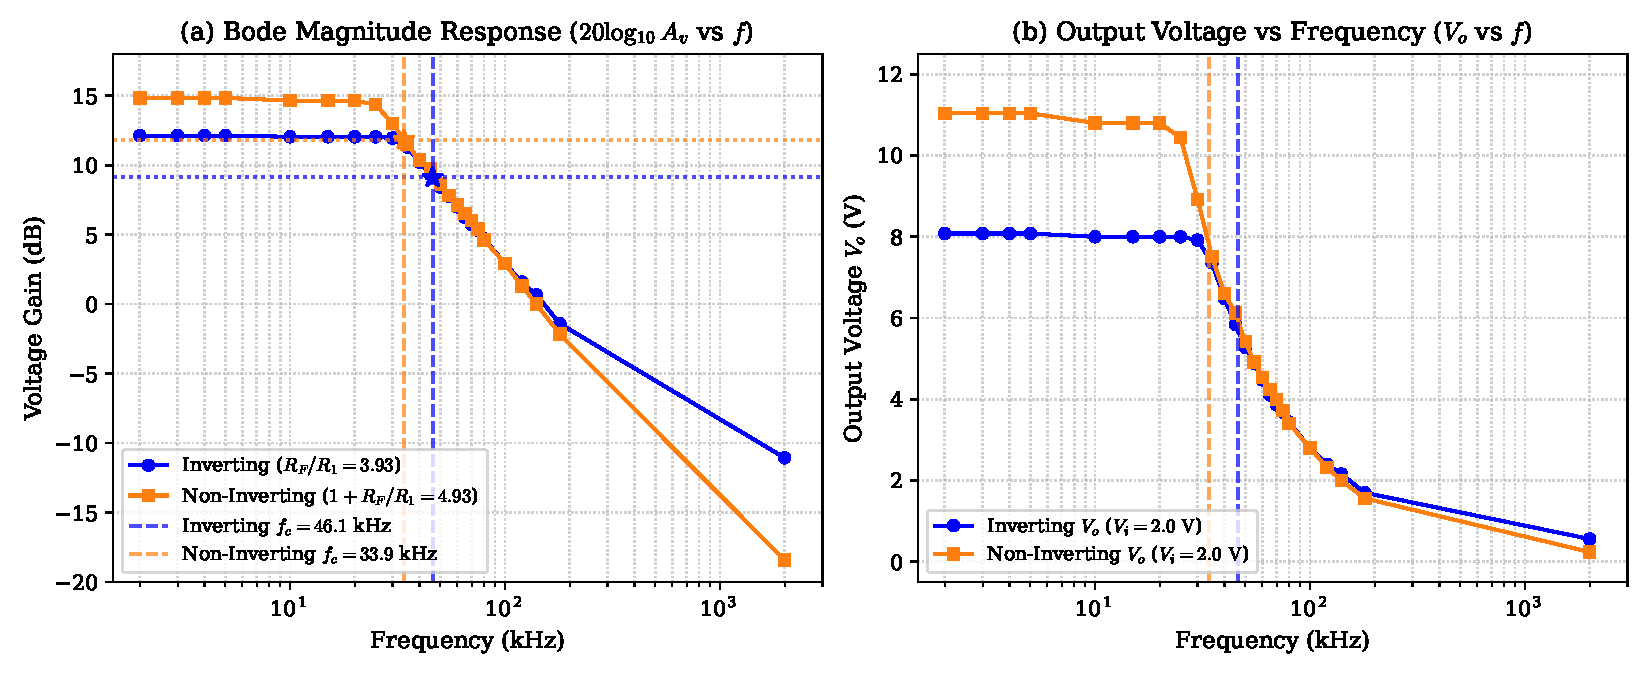
\includegraphics[width=0.96\textwidth]{frequency_response.pdf}
\caption{Frequency response of IC 741: (a) Bode magnitude plot showing midband gains, $-3\text{ dB}$ cutoff frequencies ($f_{c,\text{inv}} = 46.1\text{ kHz}$, $f_{c,\text{non}} = 33.9\text{ kHz}$), and high-frequency roll-off, and (b) peak-to-peak output voltage $V_o$ versus frequency.}
\end{figure}

\subsection{Waveform Observations for Integrator Circuit}
\begin{figure}[H]
\centering
\begin{subfigure}[b]{0.48\textwidth}
\centering
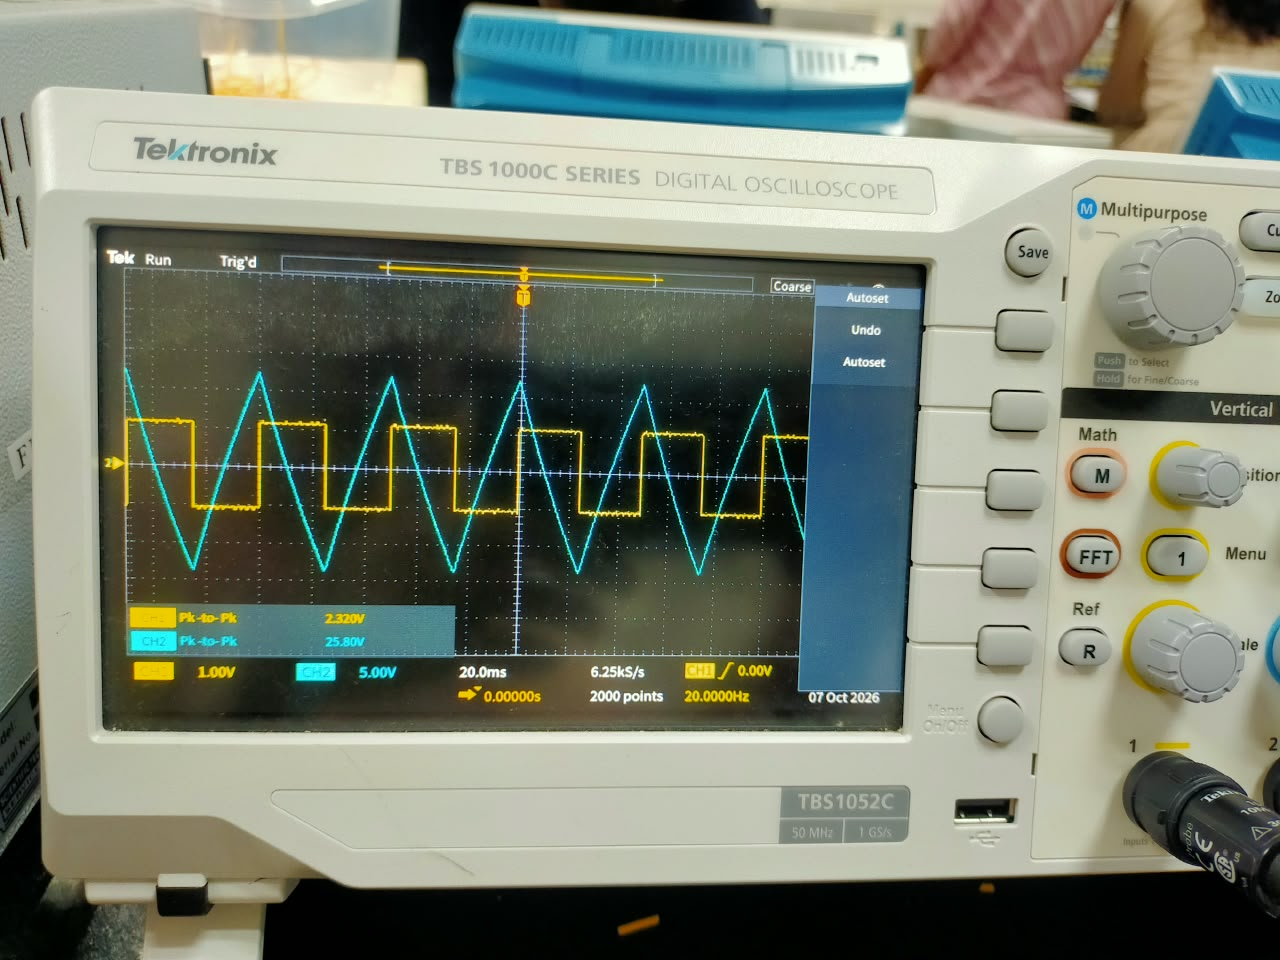
\includegraphics[width=\textwidth]{../my observations/Square wave integration.jpeg}
\caption{Square wave input ($20\text{ Hz}$, $2.32\text{ V}_{p-p}$) integrated into a triangular wave output ($25.80\text{ V}_{p-p}$).}
\end{subfigure}
\hfill
\begin{subfigure}[b]{0.48\textwidth}
\centering
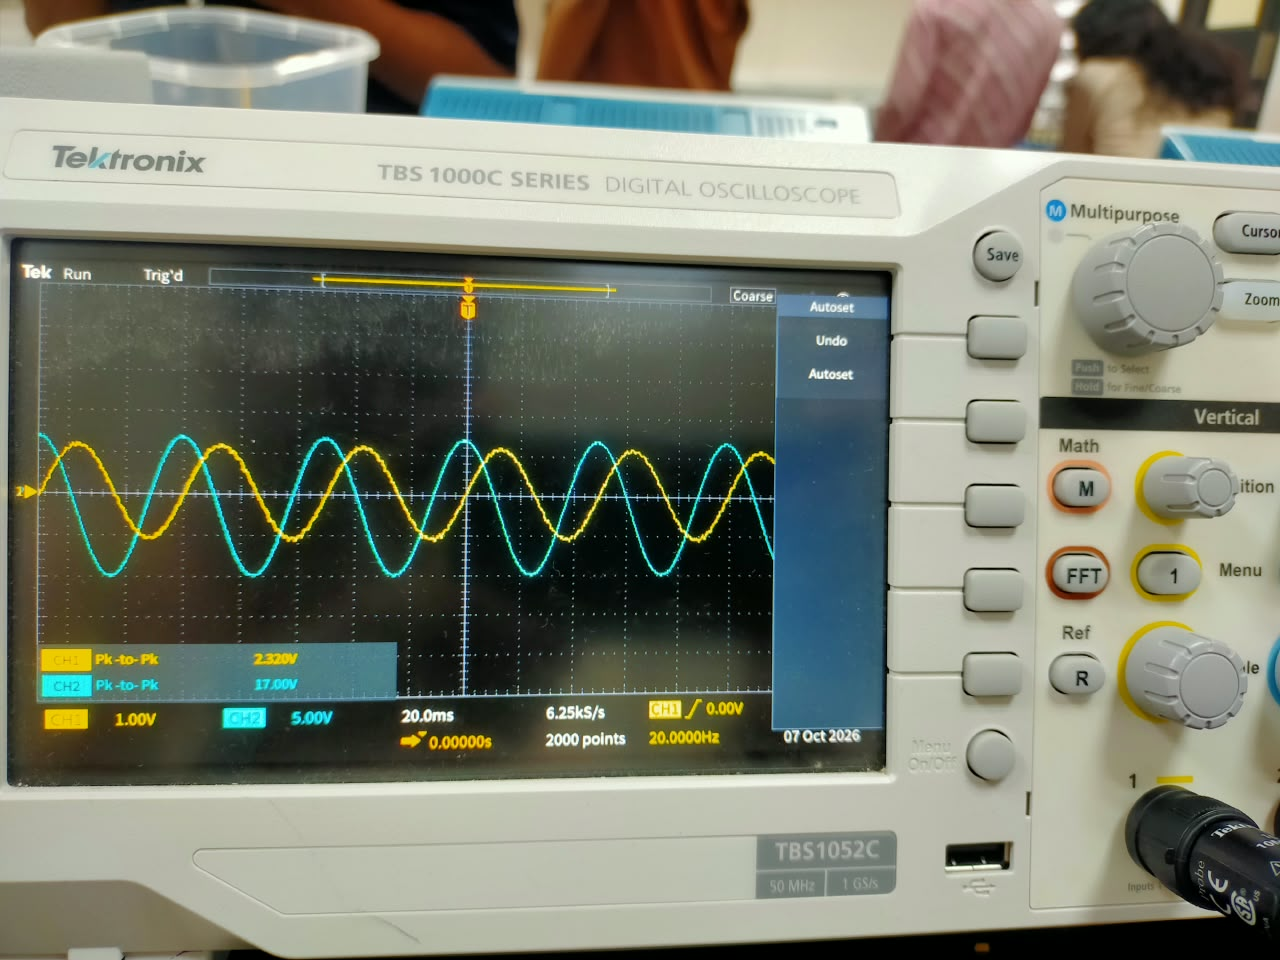
\includegraphics[width=\textwidth]{../my observations/sine wave integration.jpeg}
\caption{Sine wave input ($20\text{ Hz}$, $2.32\text{ V}_{p-p}$) integrated into a $90^\circ$ phase-shifted cosine wave ($17.00\text{ V}_{p-p}$).}
\end{subfigure}

\vspace{0.3cm}
\begin{subfigure}[b]{0.52\textwidth}
\centering
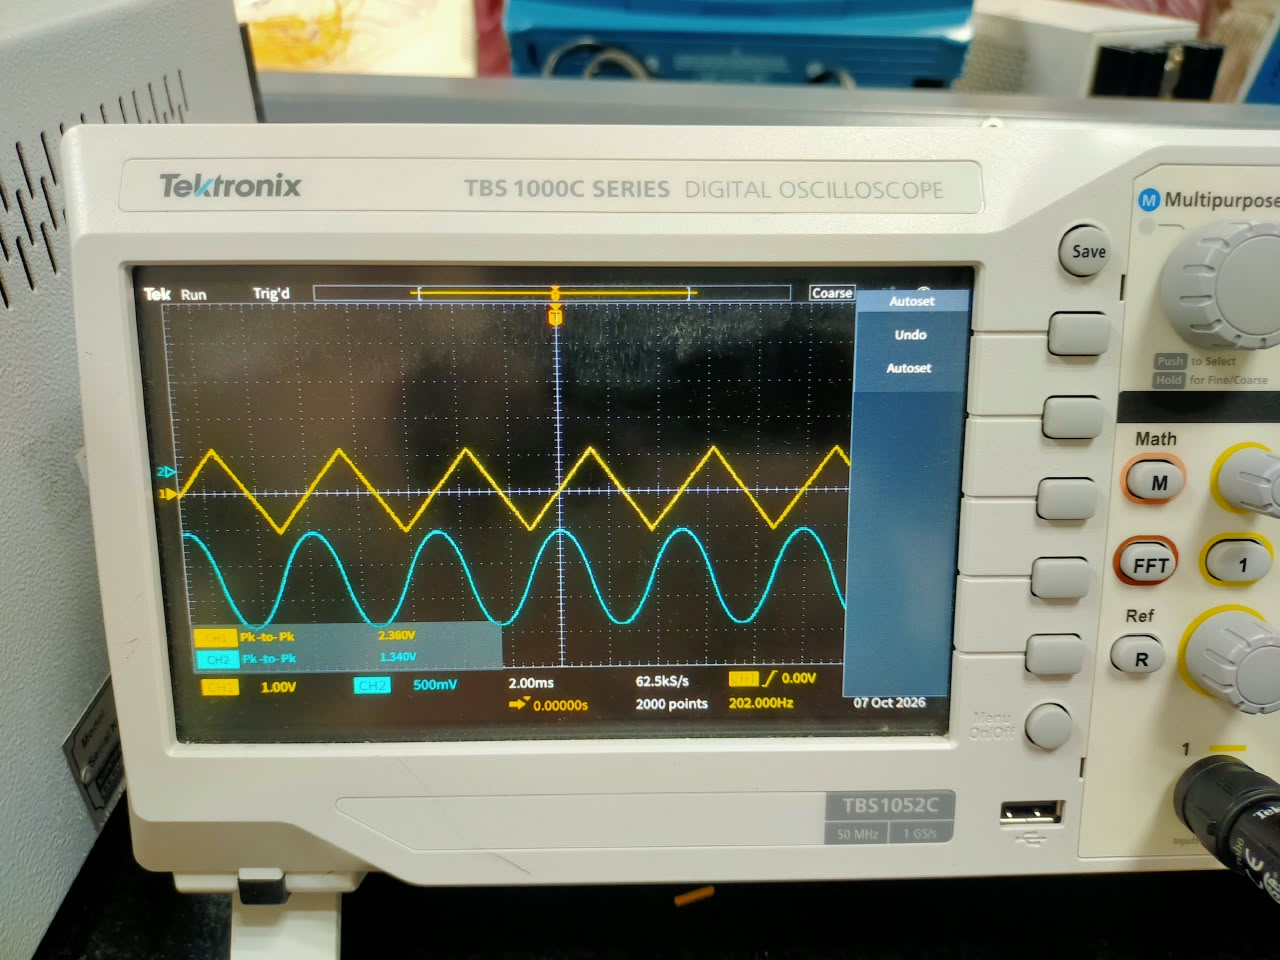
\includegraphics[width=\textwidth]{../my observations/trinagle wave integration.jpeg}
\caption{Triangle wave input ($202\text{ Hz}$, $2.36\text{ V}_{p-p}$) integrated into a smooth parabolic wave ($1.34\text{ V}_{p-p}$).}
\end{subfigure}
\caption{Oscilloscope captures for operational amplifier integrator circuit performing time integration across different input waveforms.}
\end{figure}

\subsection{Waveform Observations for Differentiator Circuit}
\begin{figure}[H]
\centering
\begin{subfigure}[b]{0.48\textwidth}
\centering
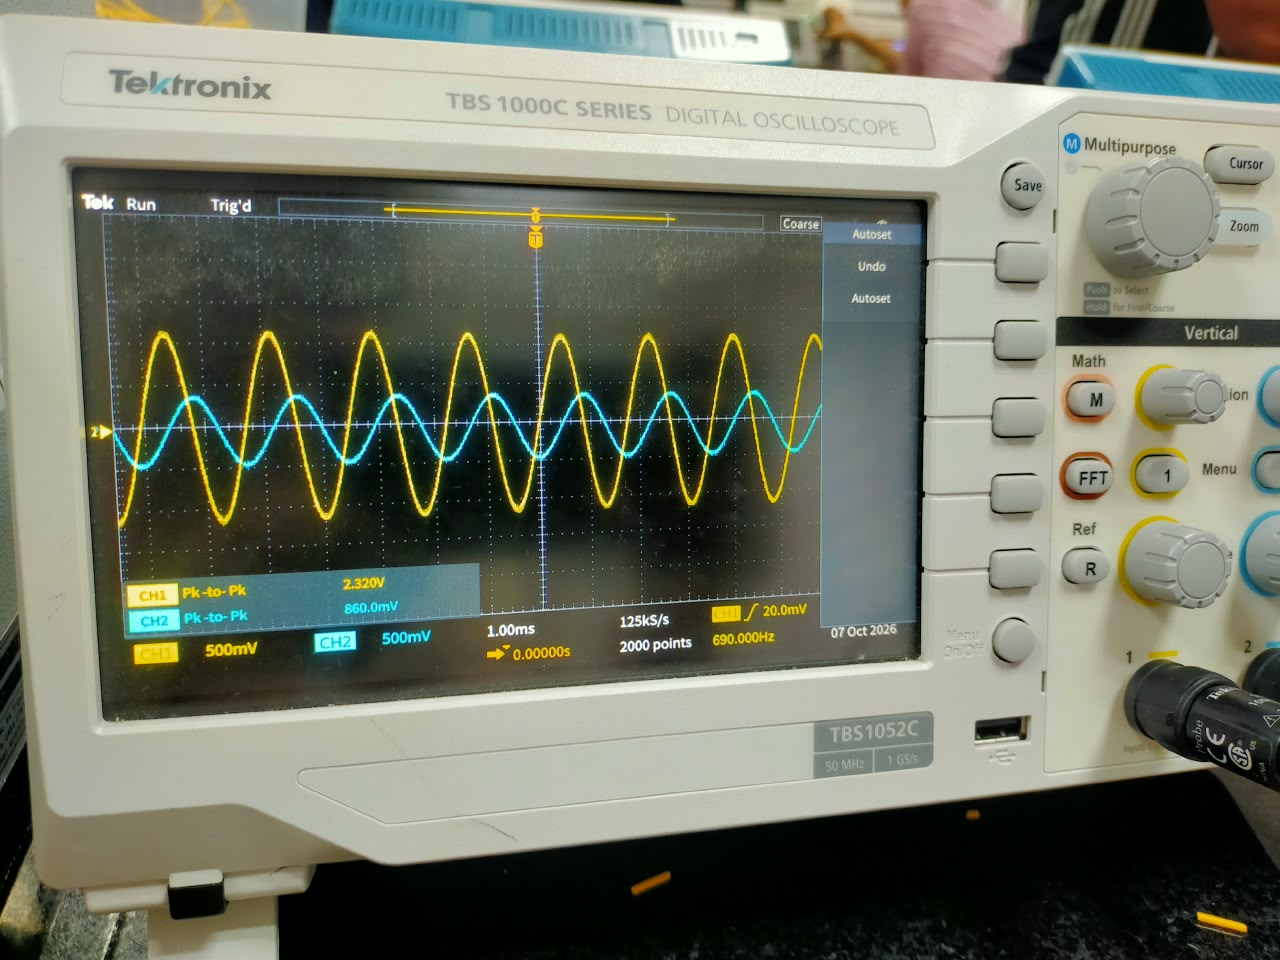
\includegraphics[width=\textwidth]{../my observations/sine wave differentation.jpeg}
\caption{Sine wave input ($690\text{ Hz}$, $2.32\text{ V}_{p-p}$) differentiated into a cosine wave ($860\text{ mV}_{p-p}$).}
\end{subfigure}
\hfill
\begin{subfigure}[b]{0.48\textwidth}
\centering
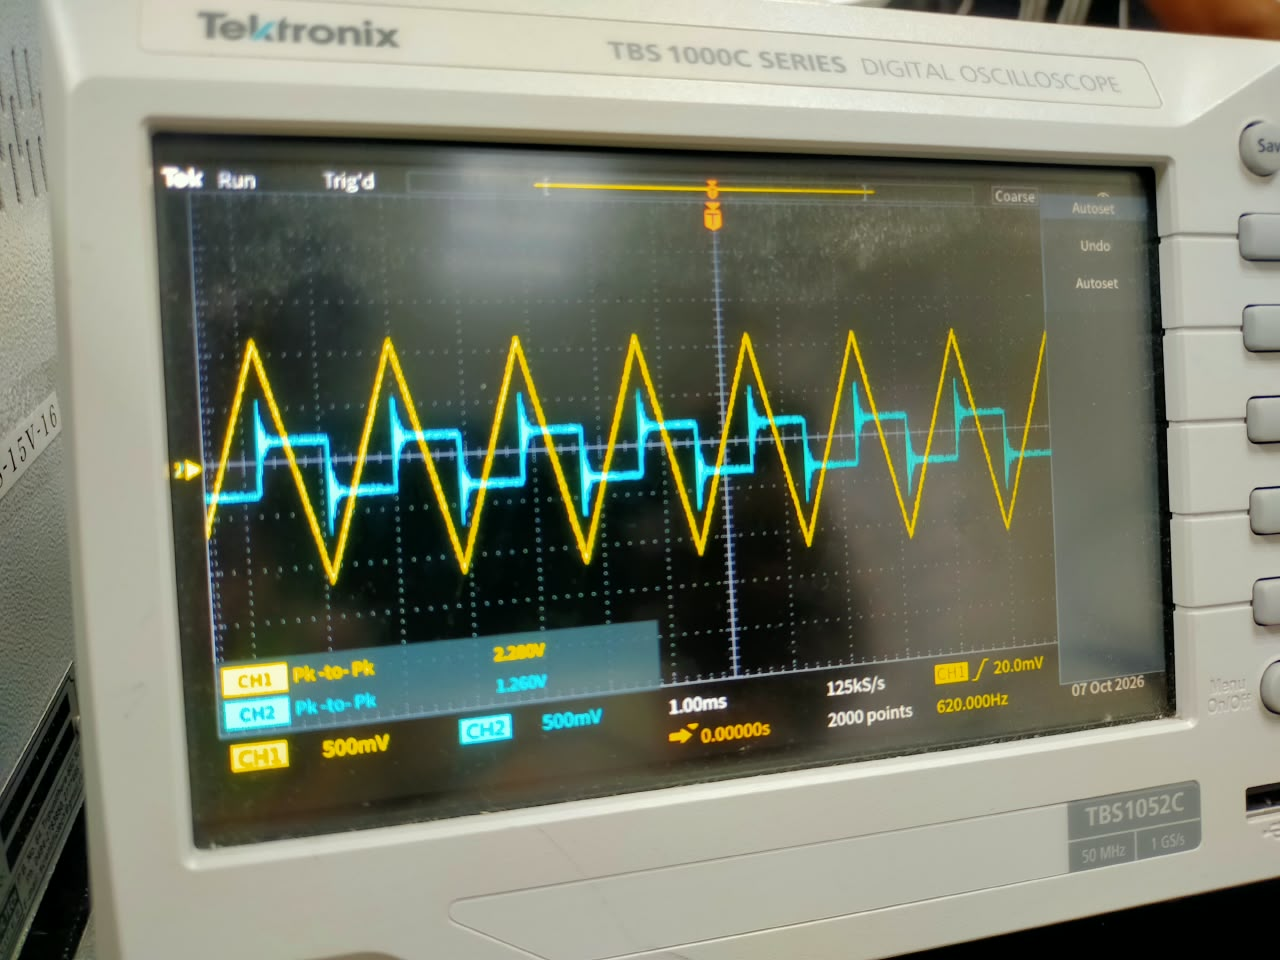
\includegraphics[width=\textwidth]{../my observations/Triangle wave differentiation.jpeg}
\caption{Triangle wave input ($620\text{ Hz}$, $2.20\text{ V}_{p-p}$) differentiated into a square wave output ($1.26\text{ V}_{p-p}$).}
\end{subfigure}
\caption{Oscilloscope captures for operational amplifier differentiator circuit performing time differentiation across sine and triangle waves.}
\end{figure}

\section{Error Calculation}

\subsection{Deviation in Voltage Gain}
Comparing theoretical and experimental midband voltage gains:
\begin{enumerate}
    \item \textbf{Inverting Amplifier:}
    \begin{equation}
        \text{Percentage Error} = \frac{|A_{v,\text{exp}} - A_{v,\text{theo}}|}{A_{v,\text{theo}}} \times 100\% = \frac{|4.04 - 3.93|}{3.93} \times 100\% \approx 2.80\%
    \end{equation}
    \item \textbf{Non-Inverting Amplifier:}
    \begin{equation}
        \text{Percentage Error} = \frac{|A_{v,\text{exp}} - A_{v,\text{theo}}|}{A_{v,\text{theo}}} \times 100\% = \frac{|5.52 - 4.93|}{4.93} \times 100\% \approx 11.9\%
    \end{equation}
\end{enumerate}

\subsection{Instrumental Uncertainty Propagation}
The resolution limits of the laboratory measurement equipment were:
\begin{itemize}
    \item Digital oscilloscope voltage measurement resolution: $\delta V_o / V_o \approx \pm 2.0\%$ ($\approx \pm 0.05\text{ V}$)
    \item Function generator input voltage amplitude uncertainty: $\delta V_i / V_i \approx \pm 2.0\%$
    \item Frequency setting uncertainty: $\delta f / f \approx \pm 1.0\%$
\end{itemize}
The fractional uncertainty in closed-loop gain $A_v = V_o / V_i$ is given by:
\begin{equation}
    \frac{\delta A_v}{A_v} = \sqrt{\left(\frac{\delta V_o}{V_o}\right)^2 + \left(\frac{\delta V_i}{V_i}\right)^2} = \sqrt{(0.02)^2 + (0.02)^2} \approx 2.83\%
\end{equation}
For the inverting amplifier ($A_{v0} = 4.04$):
\begin{equation}
    \delta A_{v,\text{inv}} = 4.04 \times 0.0283 \approx 0.11 \implies A_{v,\text{inv}} = 4.04 \pm 0.11
\end{equation}
For the non-inverting amplifier ($A_{v0} = 5.52$):
\begin{equation}
    \delta A_{v,\text{non}} = 5.52 \times 0.0283 \approx 0.16 \implies A_{v,\text{non}} = 5.52 \pm 0.16
\end{equation}
The fractional uncertainty in the Gain-Bandwidth Product is:
\begin{equation}
    \frac{\delta (\text{GBWP})}{\text{GBWP}} = \sqrt{\left(\frac{\delta A_v}{A_v}\right)^2 + \left(\frac{\delta f_c}{f_c}\right)^2} \approx \sqrt{(0.0283)^2 + (0.02)^2} \approx 3.47\%
\end{equation}
Thus, for the inverting configuration:
\begin{equation}
    \delta (\text{GBWP}) = 186.2\text{ kHz} \times 0.0347 \approx 6.5\text{ kHz} \implies \text{GBWP} = (186.2 \pm 6.5)\text{ kHz}
\end{equation}

\section{Discussion}
In this experiment, we investigated the frequency response and mathematical processing capabilities of the IC 741 operational amplifier. 

\subsection{Frequency Response and Gain-Bandwidth Conservation}
The open-loop gain of an uncompensated op-amp drops at higher frequencies due to internal parasitic capacitances. In the internally compensated IC 741, an integrated $30\text{ pF}$ MOS capacitor intentionally forces the open-loop gain to begin rolling off at around $10\text{ Hz}$ with a constant slope of $-20\text{ dB/decade}$. This deliberate attenuation ensures unconditional phase margin and stability against self-oscillation when negative feedback is applied.

When configured as closed-loop inverting and non-inverting amplifiers, the circuits exhibited flat gain across the audio frequency band up to their respective cutoff points ($46.1\text{ kHz}$ and $33.9\text{ kHz}$). Beyond these cutoff frequencies, the gain decreased linearly on the logarithmic plot at $-20\text{ dB/decade}$. Notably, the product of the midband gain and cutoff frequency remained exceptionally constant: $186.2\text{ kHz}$ for the inverting configuration versus $187.2\text{ kHz}$ for the non-inverting configuration (a discrepancy under $0.5\%$). This provides clear experimental validation that closed-loop gain can be directly exchanged for operating bandwidth.

\subsection{Mathematical Tool Operations}
The mathematical computing circuits successfully demonstrated basic analog signal processing:
\begin{itemize}
    \item \textbf{Summing and Difference Amplifiers:} Relied on the virtual ground property at the inverting node to sum and subtract voltages without mutual loading between input channels.
    \item \textbf{Active Integrator:} Successfully generated a triangular wave from a square wave, an inverted cosine wave from a sine wave, and parabolic segments from a triangular wave. The stabilizing feedback resistor $R_1$ prevented DC saturation from input bias currents and offset voltages.
    \item \textbf{Active Differentiator:} Differentiating a triangular wave produced a square wave, while differentiating a sine wave produced a cosine wave. High-frequency spikes and ringing were visible at the transition edges in the oscilloscope trace; these arise because differentiation amplifies high-frequency harmonics, and the finite slew rate of the op-amp limits how rapidly the output can swing between saturation states.
\end{itemize}

\subsection{Differences Between Theoretical Assumptions and Bench Reality}
Several non-ideal factors were noted:
\begin{itemize}
    \item \textbf{Component Tolerances:} Practical carbon and metal film resistors carry a $\pm 5\%$ tolerance, explaining the slight variance between calculated nominal gains ($3.93$ and $4.93$) and bench-measured values ($4.04$ and $5.52$).
    \item \textbf{Slew Rate Limitation:} The maximum rate of change of output voltage in IC 741 is typically $0.5\text{ V}/\mu\text{s}$. For high-frequency large-amplitude signals, output waveforms exhibit slew-rate induced distortion rather than purely sinusoidal behavior.
    \item \textbf{High-Frequency Noise in Differentiators:} Differentiator circuits naturally emphasize high-frequency noise because gain increases linearly with frequency ($\omega RC$), necessitating series input resistance in practical industrial circuits.
\end{itemize}

\section{References}
\begin{enumerate}
    \item Lab Manual for Advanced Physics Lab II, Department of Physics, IISER Thiruvananthapuram.
    \item Chattopadhyay, D., \& Rakshit, P. C., \textit{Electronics Fundamentals and Applications}, 14th Edition, New Age International Publishers, 2017.
    \item Boylestad, R. L., \& Nashelsky, L., \textit{Electronic Devices and Circuit Theory}, 11th Edition, Pearson.
    \item Sedra, A. S., \& Smith, K. C., \textit{Microelectronic Circuits}, 8th Edition, Oxford University Press.
\end{enumerate}

\section{Lab Notes (Observations)}
The following figures present the original handwritten laboratory observation sheets containing circuit diagrams, component specifications, and frequency response data recorded during the laboratory session.

\begin{figure}[H]
    \centering
    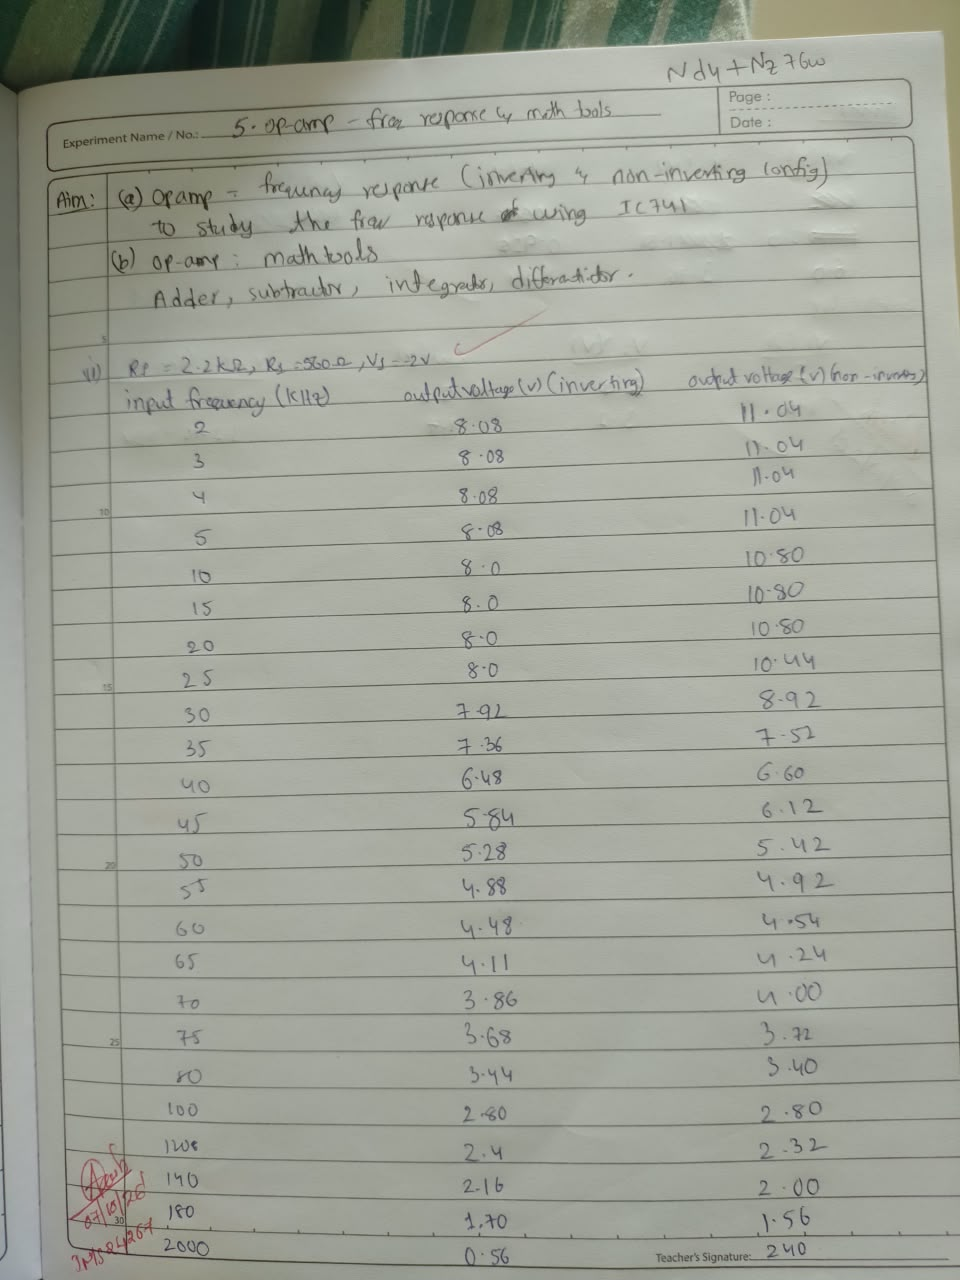
\includegraphics[height=0.72\textheight, keepaspectratio]{../my observations/1.jpeg}
    \caption{Handwritten laboratory notes: Experiment aim, circuit parameters ($R_F = 2.2\text{ k}\Omega$, $R_1 = 560\ \Omega$, $V_i = 2\text{ V}$), and frequency response observation table for inverting and non-inverting amplifiers.}
\end{figure}

\begin{figure}[H]
    \centering
    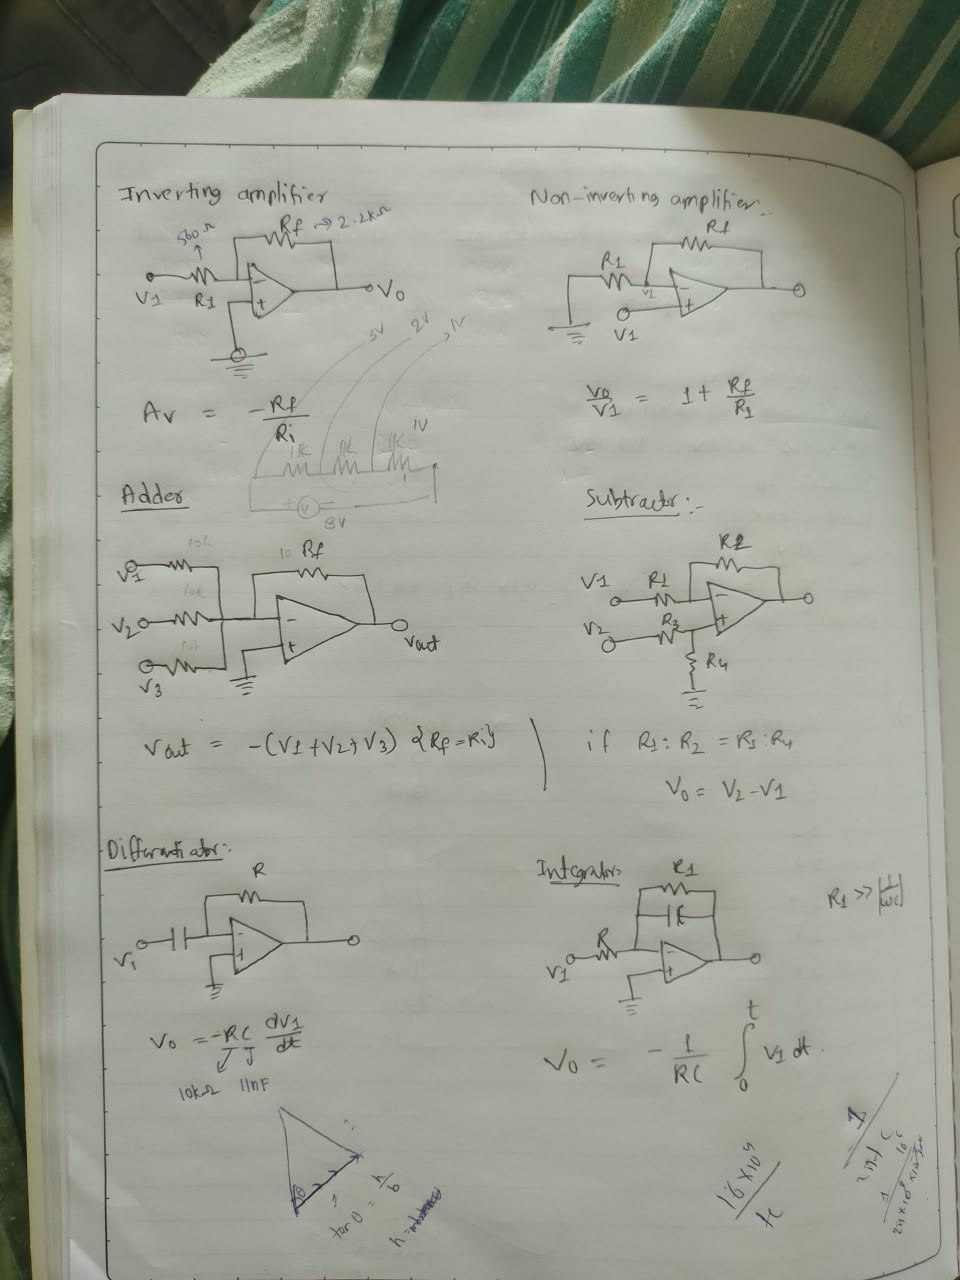
\includegraphics[height=0.72\textheight, keepaspectratio]{../my observations/2.jpeg}
    \caption{Handwritten laboratory notes: Circuit schematics for inverting amplifier, non-inverting amplifier, summing amplifier (adder), difference amplifier (subtractor), differentiator, and integrator.}
\end{figure}

\end{document}
